% $Id: $
%%\VignetteIndexEntry{Examples for kinetic evaluations using kinfit}
%%\usepackage{Sweave}
\documentclass[12pt,a4paper]{article}
\usepackage{a4wide}
%%\usepackage[lists,heads]{endfloat}
\usepackage{booktabs}
\usepackage{amsfonts}
\usepackage{latexsym}
\usepackage{amsmath}
\usepackage{amssymb}
\usepackage{graphicx}
\usepackage{parskip}
\usepackage[round]{natbib}
\usepackage{amstext}
\usepackage{hyperref}
\usepackage[utf8]{inputenc}

\newcommand{\Rpackage}[1]{{\normalfont\fontseries{b}\selectfont #1}}
\newcommand{\Robject}[1]{\texttt{#1}}
\newcommand{\Rclass}[1]{\textit{#1}}
\newcommand{\Rcmd}[1]{\texttt{#1}}

\newcommand{\RR}{\textsf{R}}

\RequirePackage[T1]{fontenc}
\RequirePackage{graphicx,ae,fancyvrb}
\IfFileExists{upquote.sty}{\RequirePackage{upquote}}{}
\usepackage{relsize}

\DefineVerbatimEnvironment{Sinput}{Verbatim}{baselinestretch=1.05}
\DefineVerbatimEnvironment{Soutput}{Verbatim}{fontfamily=courier,
                                              baselinestretch=1.05,
                                              fontshape=it,
                                              fontsize=\relsize{-1}}
\DefineVerbatimEnvironment{Scode}{Verbatim}{}  
\newenvironment{Schunk}{}{}

\hypersetup{  
  pdftitle = {Examples for kinetic evaluations using kinfit},
  pdfsubject = {Manuscript},
  pdfauthor = {Johannes Ranke},
  colorlinks = {true},
  linkcolor = {blue},
  citecolor = {blue},
  urlcolor = {red},
  hyperindex = {true},
  linktocpage = {true},
}

\begin{document}
\title{Examples for kinetic evaluations using kinfit}
\author{\textbf{Johannes Ranke} \\[0.5cm]
%EndAName
Eurofins Regulatory AG\\
Weidenweg 15, CH--4310 Rheinfelden, Switzerland\\[0.5cm]
and\\[0.5cm]
University of Bremen\\
}
\maketitle

%\begin{abstract}
%\end{abstract}

\thispagestyle{empty} \setcounter{page}{0}

\clearpage

\tableofcontents

\textbf{Key words}: Kinetics, FOCUS, nonlinear optimisation

\section{Kinetic evaluations for parent compounds}
\label{intro}

These examples are also evaluated in a parallel vignette of the
\Rpackage{mkin} package \citep{pkg:mkin}. The datasets are from Appendix 3,
of the FOCUS kinetics report \citep{FOCUS2006, FOCUSkinetics2011}.

\subsection{Laboratory Data L1}

The following code defines an object containing the example dataset L1 from the
FOCUS kinetics report, p. 284

\begin{Schunk}
\begin{Sinput}
R> library("kinfit")
R> FOCUS_2006_L1 = kinobject("Parent", "Degradation data", "")
R> FOCUS_2006_L1$data = data.frame(
+   t = rep(c(0, 1, 2, 3, 5, 7, 14, 21, 30), each = 2),
+   parent = c(88.3, 91.4, 85.6, 84.5, 78.9, 77.6, 
+              72.0, 71.9, 50.3, 59.4, 47.0, 45.1,
+              27.7, 27.3, 10.0, 10.4, 2.9, 4.0))
\end{Sinput}
\end{Schunk}

The following two lines fit the model and produce the summary report
of the model fit. This covers the numerical analyses given in the 
FOCUS report.

\begin{Schunk}
\begin{Sinput}
R> FOCUS_2006_L1$fits <- kinfit(FOCUS_2006_L1$data, 
+   kinmodels = c("SFO", "FOMC", "DFOP"))
R> FOCUS_2006_L1$results <- kinresults(FOCUS_2006_L1$fits)
R> kinreport(FOCUS_2006_L1)
\end{Sinput}
\begin{Soutput}
Parent compound:  Parent 
Study type:       Degradation data 
System:            
kinfit version:   1.1.10 
R version:        2.15.2 
Report generated: Sun Feb 17 21:07:59 2013 

Data:
    t parent
1   0   88.3
2   0   91.4
3   1   85.6
4   1   84.5
5   2   78.9
6   2   77.6
7   3   72.0
8   3   71.9
9   5   50.3
10  5   59.4
11  7   47.0
12  7   45.1
13 14   27.7
14 14   27.3
15 21   10.0
16 21   10.4
17 30    2.9
18 30    4.0



---
Nonlinear least squares fit of the SFO model

Parameter estimation:	
         Estimate Std. Error t value   Pr(>t)
parent.0  92.4710    1.36830    67.6 0.00e+00
k          0.0956    0.00388    24.6 1.87e-14

Chi2 error estimation: 3.42 %



---
Endpoint estimates

    DT50 DT90
SFO  7.2 24.1
\end{Soutput}
\end{Schunk}

Obviously, the FOMC model and the DFOP model were not fitted. As discussed in the
kinfit vignette of this package, this occurs when the SFO model fits very well.

We can try to force the FOMC fit using the parameters obtained using mkin.

\begin{Schunk}
\begin{Sinput}
R> FOCUS_2006_L1$fits <- kinfit(FOCUS_2006_L1$data, 
+   kinmodels = c("SFO", "FOMC", "DFOP"),
+   start.FOMC = list(parent.0 = 92.47, alpha = 1.35e11, beta = 1.41e12))
R> FOCUS_2006_L1$results <- kinresults(FOCUS_2006_L1$fits)
R> kinreport(FOCUS_2006_L1)
\end{Sinput}
\begin{Soutput}
Parent compound:  Parent 
Study type:       Degradation data 
System:            
kinfit version:   1.1.10 
R version:        2.15.2 
Report generated: Sun Feb 17 21:08:00 2013 

Data:
    t parent
1   0   88.3
2   0   91.4
3   1   85.6
4   1   84.5
5   2   78.9
6   2   77.6
7   3   72.0
8   3   71.9
9   5   50.3
10  5   59.4
11  7   47.0
12  7   45.1
13 14   27.7
14 14   27.3
15 21   10.0
16 21   10.4
17 30    2.9
18 30    4.0



---
Nonlinear least squares fit of the SFO model

Parameter estimation:	
         Estimate Std. Error t value   Pr(>t)
parent.0  92.4710    1.36830    67.6 0.00e+00
k          0.0956    0.00388    24.6 1.87e-14

Chi2 error estimation: 3.42 %



---
Endpoint estimates

    DT50 DT90
SFO  7.2 24.1
\end{Soutput}
\end{Schunk}

It still does not converge. As discussed in the kinfit vignette, the FOMC model usually
is not returned by kinfit when the SFO model fits very well. This should be seen as 
a feature, not a bug, as the FOMC model is ill-defined in such cases.

A plot of the fit is obtained with the kinplot function.

\begin{Schunk}
\begin{Sinput}
R> kinplot(FOCUS_2006_L1, ylab = "Observed")
\end{Sinput}
\end{Schunk}
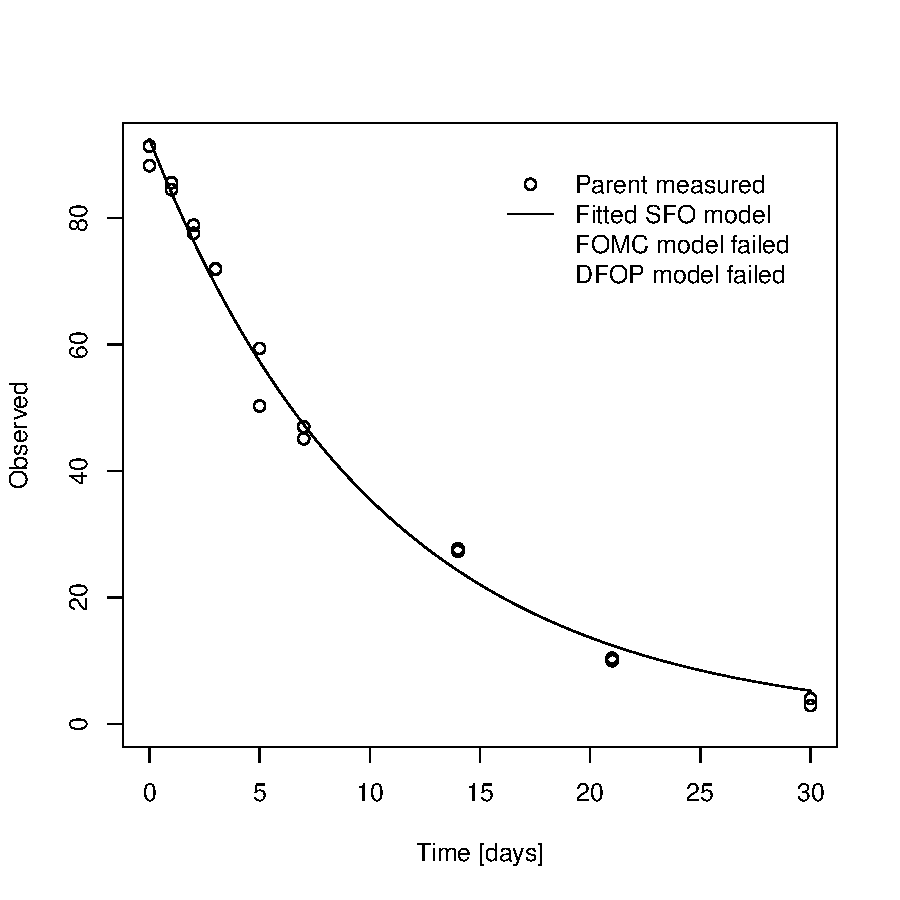
\includegraphics{examples-L1_SFO_plot}

The residual plot can be easily obtained by

\begin{Schunk}
\begin{Sinput}
R> kinresplot(FOCUS_2006_L1, "SFO", ylab = "Observed")
\end{Sinput}
\end{Schunk}
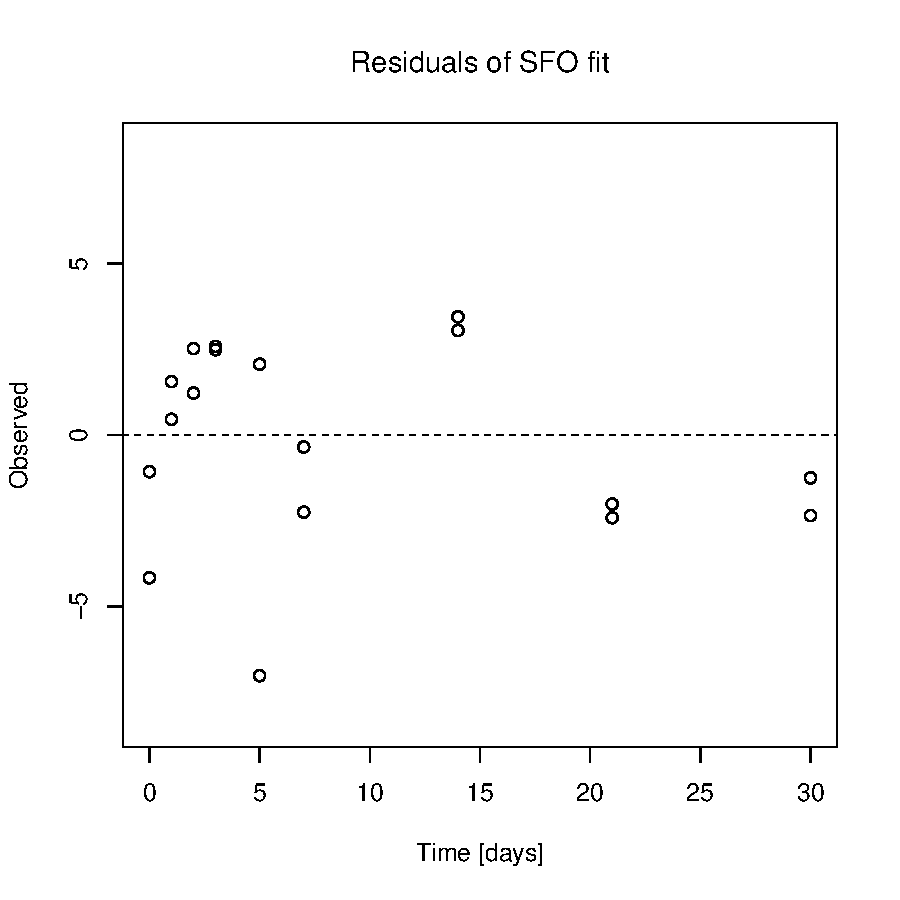
\includegraphics{examples-L1_SFO_residuals}

\subsection{Laboratory Data L2}

The following code defines example dataset L2 from the FOCUS kinetics
report, p. 287

\begin{Schunk}
\begin{Sinput}
R> FOCUS_2006_L2 = kinobject("Parent", "Degradation data", "")
R> FOCUS_2006_L2$data = data.frame(
+   t = rep(c(0, 1, 3, 7, 14, 28), each = 2),
+   parent = c(96.1, 91.8, 41.4, 38.7,
+              19.3, 22.3, 4.6, 4.6,
+              2.6, 1.2, 0.3, 0.6))
\end{Sinput}
\end{Schunk}

Again, the SFO, FOMC and DFOP models are fitted and a report is printed.

\begin{Schunk}
\begin{Sinput}
R> FOCUS_2006_L2$fits <- kinfit(FOCUS_2006_L2$data, 
+   kinmodels = c("SFO", "FOMC", "DFOP"))
R> FOCUS_2006_L2$results <- kinresults(FOCUS_2006_L2$fits)
R> kinreport(FOCUS_2006_L2)
\end{Sinput}
\begin{Soutput}
Parent compound:  Parent 
Study type:       Degradation data 
System:            
kinfit version:   1.1.10 
R version:        2.15.2 
Report generated: Sun Feb 17 21:08:00 2013 

Data:
    t parent
1   0   96.1
2   0   91.8
3   1   41.4
4   1   38.7
5   3   19.3
6   3   22.3
7   7    4.6
8   7    4.6
9  14    2.6
10 14    1.2
11 28    0.3
12 28    0.6



---
Nonlinear least squares fit of the SFO model

Parameter estimation:	
         Estimate Std. Error t value   Pr(>t)
parent.0   91.466     3.8065   24.03 1.77e-10
k           0.663     0.0712    9.31 1.52e-06

Chi2 error estimation: 14.38 %



---
Nonlinear least squares fit of the FOMC model

Parameter estimation:	
         Estimate Std. Error t value   Pr(>t)
parent.0    93.77      1.856   50.51 1.17e-12
alpha        1.37      0.257    5.36 2.30e-04
beta         1.23      0.363    3.40 3.95e-03

Chi2 error estimation: 6.2 %



---
Endpoint estimates

     DT50 DT90
SFO   1.0  3.5
FOMC  0.8  5.4
\end{Soutput}
\end{Schunk}

Here, only the DFOP did not converge using default parameters. The DFOP fit can be 
obtained using refined starting parameters:

\begin{Schunk}
\begin{Sinput}
R> FOCUS_2006_L2$fits <- kinfit(FOCUS_2006_L2$data, 
+   kinmodels = c("SFO", "FOMC", "DFOP"),
+   start.DFOP = list(parent.0 = 94, g = 0.4, k1 = 142, k2 = 0.34))
R> FOCUS_2006_L2$results <- kinresults(FOCUS_2006_L2$fits)
R> kinreport(FOCUS_2006_L2)
\end{Sinput}
\begin{Soutput}
Parent compound:  Parent 
Study type:       Degradation data 
System:            
kinfit version:   1.1.10 
R version:        2.15.2 
Report generated: Sun Feb 17 21:08:00 2013 

Data:
    t parent
1   0   96.1
2   0   91.8
3   1   41.4
4   1   38.7
5   3   19.3
6   3   22.3
7   7    4.6
8   7    4.6
9  14    2.6
10 14    1.2
11 28    0.3
12 28    0.6



---
Nonlinear least squares fit of the SFO model

Parameter estimation:	
         Estimate Std. Error t value   Pr(>t)
parent.0   91.466     3.8065   24.03 1.77e-10
k           0.663     0.0712    9.31 1.52e-06

Chi2 error estimation: 14.38 %



---
Nonlinear least squares fit of the FOMC model

Parameter estimation:	
         Estimate Std. Error t value   Pr(>t)
parent.0    93.77      1.856   50.51 1.17e-12
alpha        1.37      0.257    5.36 2.30e-04
beta         1.23      0.363    3.40 3.95e-03

Chi2 error estimation: 6.2 %



---
Endpoint estimates

     DT50 DT90
SFO   1.0  3.5
FOMC  0.8  5.4
\end{Soutput}
\end{Schunk}

Again, even with starting parameters very close to the optimum obtained using mkin, 
there is no convergence with kinfit. However, when looking at the fit obtained using
mkin plotted in the mkin vignette, it is clear that the point where the break point 
of the curve, caused by the large difference between k1 and k2, is not clearly defined
by the data. Therefore, it should be seen as a desirable feature of the
underlying nls() function that no solution is returned.

Comparison of $\chi^2$ error levels of the two models shows that the FOMC model allows
for a better representation of the data.  This is also obvious from the plot
of the fits.

\begin{Schunk}
\begin{Sinput}
R> kinplot(FOCUS_2006_L2, ylab = "Observed")
\end{Sinput}
\end{Schunk}
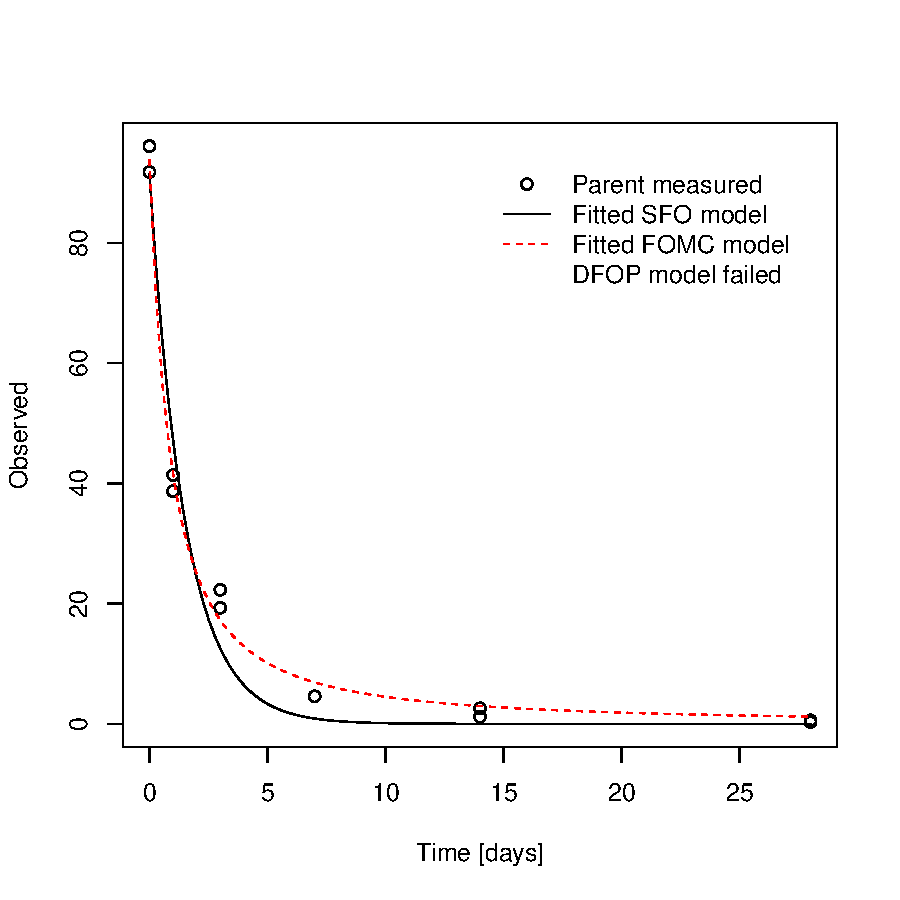
\includegraphics{examples-L2_plot}

Residual plots are obtained using kinresplot.

\begin{Schunk}
\begin{Sinput}
R> par(mfrow=c(2,1))
R> kinresplot(FOCUS_2006_L2, "SFO", ylab = "Observed")
R> kinresplot(FOCUS_2006_L2, "FOMC", ylab = "Observed")
\end{Sinput}
\end{Schunk}
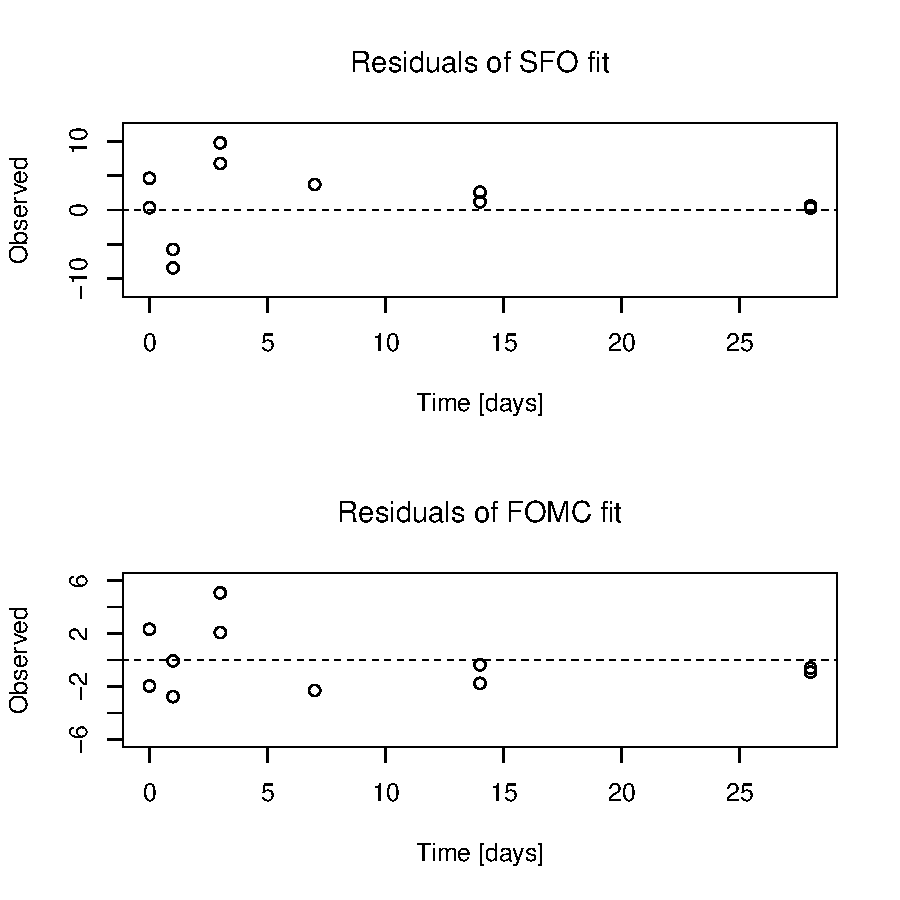
\includegraphics{examples-L2_resplot}

\subsection{Laboratory Data L3}

The following code defines example dataset L3 from the FOCUS kinetics
report, p. 290 and attempts to fit the SFO, FOMC and DFOP models.

\begin{Schunk}
\begin{Sinput}
R> FOCUS_2006_L3 = kinobject("Parent", "Degradation data", "")
R> FOCUS_2006_L3$data = data.frame(
+   t = c(0, 3, 7, 14, 30, 60, 91, 120),
+   parent = c(97.8, 60, 51, 43, 35, 22, 15, 12))
R> FOCUS_2006_L3$fits <- kinfit(FOCUS_2006_L3$data, 
+   kinmodels = c("SFO", "FOMC", "DFOP"))
R> FOCUS_2006_L3$results <- kinresults(FOCUS_2006_L3$fits)
R> kinreport(FOCUS_2006_L3)
\end{Sinput}
\begin{Soutput}
Parent compound:  Parent 
Study type:       Degradation data 
System:            
kinfit version:   1.1.10 
R version:        2.15.2 
Report generated: Sun Feb 17 21:08:00 2013 

Data:
    t parent
1   0   97.8
2   3   60.0
3   7   51.0
4  14   43.0
5  30   35.0
6  60   22.0
7  91   15.0
8 120   12.0



---
Nonlinear least squares fit of the SFO model

Parameter estimation:	
         Estimate Std. Error t value   Pr(>t)
parent.0  74.8718    8.45736    8.85 5.78e-05
k          0.0253    0.00824    3.07 1.10e-02

Chi2 error estimation: 21.24 %



---
Nonlinear least squares fit of the DFOP model

Parameter estimation:	
         Estimate Std. Error t value   Pr(>t)
parent.0  97.7460   1.438160    68.0 1.40e-07
k1         0.5162   0.068841     7.5 8.46e-04
k2         0.0138   0.000812    16.9 3.56e-05
g          0.4566   0.017970    25.4 7.12e-06

Chi2 error estimation: 2.22 %



---
Endpoint estimates

     DT50  DT90
SFO  27.4  91.1
DFOP  7.5 123.0
\end{Soutput}
\end{Schunk}

In this case, the FOMC model does not return a solution using kinfit. Trying with 
closer starting parameters gives success this time.

\begin{Schunk}
\begin{Sinput}
R> FOCUS_2006_L3$fits <- kinfit(FOCUS_2006_L3$data, 
+   kinmodels = c("SFO", "FOMC", "DFOP"),
+   start.FOMC = list(parent.0 = 100, alpha = 0.5, beta = 2))
R> FOCUS_2006_L3$results <- kinresults(FOCUS_2006_L3$fits)
R> kinreport(FOCUS_2006_L3)
\end{Sinput}
\begin{Soutput}
Parent compound:  Parent 
Study type:       Degradation data 
System:            
kinfit version:   1.1.10 
R version:        2.15.2 
Report generated: Sun Feb 17 21:08:00 2013 

Data:
    t parent
1   0   97.8
2   3   60.0
3   7   51.0
4  14   43.0
5  30   35.0
6  60   22.0
7  91   15.0
8 120   12.0



---
Nonlinear least squares fit of the SFO model

Parameter estimation:	
         Estimate Std. Error t value   Pr(>t)
parent.0  74.8718    8.45736    8.85 5.78e-05
k          0.0253    0.00824    3.07 1.10e-02

Chi2 error estimation: 21.24 %



---
Nonlinear least squares fit of the FOMC model

Parameter estimation:	
         Estimate Std. Error t value   Pr(>t)
parent.0   96.974      4.550   21.31 2.11e-06
alpha       0.422      0.072    5.87 1.02e-03
beta        1.858      0.881    2.11 4.44e-02

Chi2 error estimation: 7.32 %



---
Nonlinear least squares fit of the DFOP model

Parameter estimation:	
         Estimate Std. Error t value   Pr(>t)
parent.0  97.7460   1.438160    68.0 1.40e-07
k1         0.5162   0.068841     7.5 8.46e-04
k2         0.0138   0.000812    16.9 3.56e-05
g          0.4566   0.017970    25.4 7.12e-06

Chi2 error estimation: 2.22 %



---
Endpoint estimates

     DT50  DT90
SFO  27.4  91.1
FOMC  7.7 431.2
DFOP  7.5 123.0
\end{Soutput}
\begin{Sinput}
R> kinplot(FOCUS_2006_L3, ylab = "Observed")
\end{Sinput}
\end{Schunk}
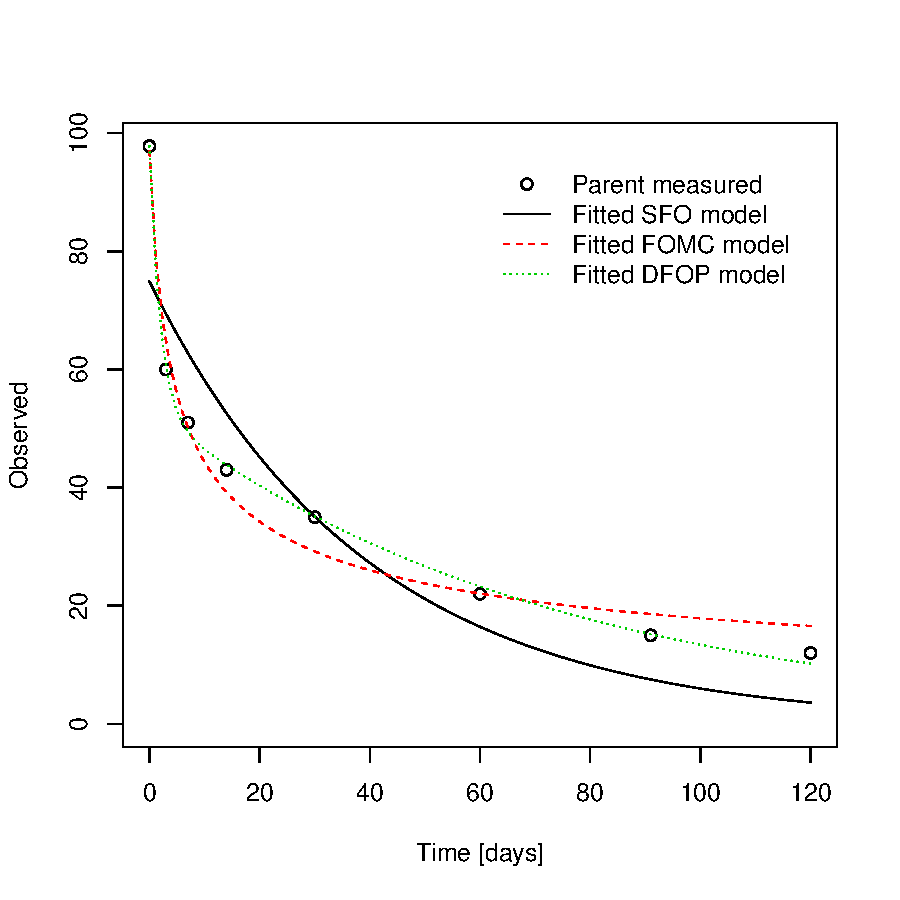
\includegraphics{examples-FOCUS_2006_L3_2}

Based on the $\chi^2$ error level criterion and the visual analysis of the
fits, the DFOP model would be the best-fit model of choice for laboratory data
L3.

\subsection{Laboratory Data L4}

The following code defines example dataset L4 from the FOCUS kinetics
report, p. 293 and attempts to fit the SFO, FOMC and DFOP models.

\begin{Schunk}
\begin{Sinput}
R> FOCUS_2006_L4 = kinobject("Parent", "Degradation data", "")
R> FOCUS_2006_L4$data = data.frame(
+   t = c(0, 3, 7, 14, 30, 60, 91, 120),
+   parent = c(96.6, 96.3, 94.3, 88.8, 74.9, 59.9, 53.5, 49.0))
R> FOCUS_2006_L4$fits <- kinfit(FOCUS_2006_L4$data, 
+   kinmodels = c("SFO", "FOMC", "DFOP"))
R> FOCUS_2006_L4$results <- kinresults(FOCUS_2006_L4$fits)
R> kinreport(FOCUS_2006_L4)
\end{Sinput}
\begin{Soutput}
Parent compound:  Parent 
Study type:       Degradation data 
System:            
kinfit version:   1.1.10 
R version:        2.15.2 
Report generated: Sun Feb 17 21:08:00 2013 

Data:
    t parent
1   0   96.6
2   3   96.3
3   7   94.3
4  14   88.8
5  30   74.9
6  60   59.9
7  91   53.5
8 120   49.0



---
Nonlinear least squares fit of the SFO model

Parameter estimation:	
         Estimate Std. Error t value   Pr(>t)
parent.0 96.44152   1.948781    49.5 2.28e-09
k         0.00654   0.000523    12.5 8.01e-06

Chi2 error estimation: 3.29 %



---
Nonlinear least squares fit of the FOMC model

Parameter estimation:	
         Estimate Std. Error t value   Pr(>t)
parent.0   99.143      1.680   59.02 1.32e-08
alpha       0.704      0.262    2.68 2.18e-02
beta       64.980     36.617    1.77 6.81e-02

Chi2 error estimation: 2.03 %



---
Nonlinear least squares fit of the DFOP model

Parameter estimation:	
         Estimate Std. Error t value   Pr(>t)
parent.0  98.7514    1.33707  73.857 1.01e-07
k1         0.0105    0.00449   2.348 3.93e-02
k2        -0.0112    0.01884  -0.596 7.08e-01
g          0.9390    0.18530   5.068 3.57e-03

Chi2 error estimation: 1.63 %



---
Endpoint estimates

      DT50   DT90
SFO  106.0  352.0
FOMC 108.9 1644.1
DFOP 118.7  122.8
\end{Soutput}
\begin{Sinput}
R> kinplot(FOCUS_2006_L4, ylab = "Observed")
\end{Sinput}
\end{Schunk}
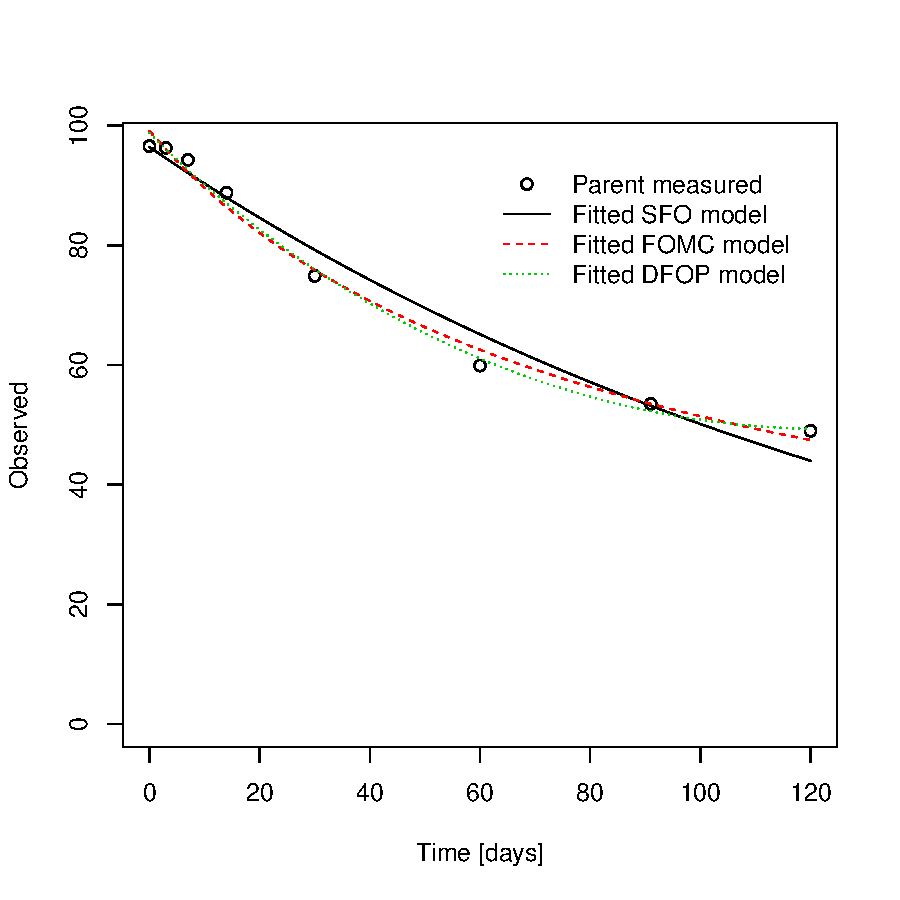
\includegraphics{examples-FOCUS_2006_L4}

Although the $\chi^2$ error level is slightly smaller for the DFOP model and also
for the FOMC model, the differences are small, and the SFO model may appear to
be a suitable choice. The better fit of the DFOP model depends very much on the
last three data points.

\bibliographystyle{plainnat}
\bibliography{references}

\end{document}
% vim: set foldmethod=syntax:
